
The testing described in Section \ref{sec:randerr} describes the process of
evaluating the methodology with test cases drawn from the training database.
It is also helpful to test the methodology against real assays of \gls{SNF}.
The \gls{SFCOMPO} database was created to allow access to these sorts of
measurements linked to the reactor operation parameters being predicted in this
work. \cite{sfcompo}. The only parameter not part of the \gls{SFCOMPO} database
is the time since irradiation, so that is not predicted here. 

\begin{figure}[!htb]
  \centering
  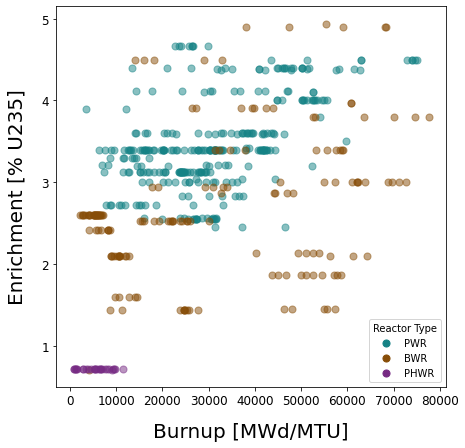
\includegraphics[width=0.7\textwidth]{./chapters/exp1/sfcompo_scatter_viz.png}
  \caption{Scatter plot showing the range of reactor operation parameters in 
           the \gls{SFCOMPO} testing set that are being predicted.}
  \label{fig:sfcoscatter}
  \todo[inline]{maybe show comparison against training E v B scatter plot}
\end{figure}

There are 505 test cases that are able to be compared against the training
database.  The number of each reactor type is as follows: 312 \gls{PWR}s, 165
\gls{BWR}s, and 28 \gls{PHWR}s. The space of enrichment and burnup values is
visualized in Figure \ref{fig:sfcoscatter}. These are sufficiently represented
in the training set design, as pictured in Figure \ref{fig:trainhist}, although
the proportions of \gls{PWR} and \gls{BWR} are approximately opposite to the
training set.

There is one main issue with using \gls{SFCOMPO} as a testing set: missing
nuclide measurements.  The feature set of 29 nuclides in Table
\ref{tbl:nucmass} was chosen based on the frequency of these measurements being
present in the database at an arbitrary level of 100 measurements. This
happened before filtering, so there are some nuclide measurements present at
under 100 counts.  Each nuclide's frequency in \gls{SFCOMPO} is listed in Table
\ref{tbl:missing}.  While every assay contains several plutonium measurements
and most contain uranium measurements as well, the remaining nuclides are
present at a much lower rate. 

\begin{table}[!htb]
  \centering
  \begin{tabular}{>{\raggedleft}m{0.6in}
                                m{0.4in}
                  >{\raggedleft}m{0.6in}
                                m{0.4in}
                  >{\raggedleft}m{0.6in}
                                m{0.4in}}
    \toprule
    \rowcolor[gray]{0.88} am241  & 237 & nd145 & 162 & sm147 & 97  \\  
    \rowcolor[gray]{0.95} am242m & 110 & nd146 & 139 & sm149 & 97  \\ 
    \rowcolor[gray]{0.88} am243  & 203 & nd148 & 275 & sm150 & 97  \\ 
    \rowcolor[gray]{0.95} cm242  & 214 & nd150 & 121 & sm151 & 97  \\ 
    \rowcolor[gray]{0.88} cm244  & 269 & np237 & 155 & sm152 & 97  \\ 
    \rowcolor[gray]{0.95} cs134  & 113 & pu238 & 369 & u234  & 355 \\ 
    \rowcolor[gray]{0.88} cs137  & 185 & pu239 & 505 & u235  & 479 \\ 
    \rowcolor[gray]{0.95} eu154  & 100 & pu240 & 505 & u236  & 462 \\ 
    \rowcolor[gray]{0.88} nd143  & 162 & pu241 & 504 & u238  & 433 \\ 
    \rowcolor[gray]{0.95} nd144  & 113 & pu242 & 505 &       &     \\ \bottomrule
  \end{tabular}
  \caption{Number of assays each nuclide is measured for in the \gls{SFCOMPO}
           database.}
  \label{tbl:missing}
\end{table}

Although some algorithms in theory can handle null values in the training
stage, scikit-learn does not currently include this capability. The \gls{MLL}
method is designed to handle null values, however. This is done by converting
them to zero and filtering out all zero-valued nuclides during the likelihood
calculations. But there is a technique more commonly applied than converting
missing values to zero: imputation. This involves taking the mean or median of
the existing features and applying that value to the assays in which it is
missing.  The remainder of this section dicusses using the three algorithms to
predict the \gls{SFCOMPO} test cases where the nulls are both converted to zero
and imputed using the mean.  \todo[inline]{is converting to zero technically
imputation as well?}

Table \ref{tbl:sfcorxtr} presents two metrics for the two missing value
techniques: the accuracy and balanced accuracy scores. The accuracy scores for
both the imputed nulls and zero-nulls test sets are mostly under 0.62, which is
the fraction of \gls{PWR} entries.  Therefore, a classifier could predict
\gls{PWR} every time and do better than these accuracy scores.  For the
zero-nulls test set predictions using \gls{MLL}, however, the accuracy of 0.72
does exceed the "majority guess" accuracy of 0.62.  Since \gls{MLL}
calculations filter out null values, it is expected that the scores will be
higher for all prediction categories where \gls{MLL} is being used with the
zero-nulls test set. This expected \gls{MLL} performance also holds true when
looking at the balanced accuracy score.  A value of 0 balanced accuracy denotes
random guessing, but it can also be negative if the classifications are worse
than random guessing. The balanced accuracy of 0.63 for the zero-nulls case is
a promising result. The balanced accuracies of \textit{k}-nearest neighbors and
decision trees are all quite low. Also, the higher accuracies correspond to lower
balanced accuracies, and vice versa. Therefore, further investigation is
necessary.

\begin{table}[!htb]
  \centering
  \begin{tabular}{@{}m{1.5in}llllll@{}}
    \toprule
    & \multicolumn{3}{m{2in}}{Accuracy Scores} 
    & \multicolumn{3}{l}{Balanced Accuracy Scores} \\ 
    \toprule
    Null Handling    & kNN   & DTree  & MLL   & kNN   & DTree  & MLL    \\ \midrule
    Imputed Nulls    & 0.52  & 0.60   & 0.39  & 0.09  & 0.12   & -0.01  \\
    Zero-value Nulls & 0.45  & 0.42   & 0.72  & 0.21  & 0.30   & 0.63   \\ \bottomrule
    \end{tabular}
  \caption{Accuracy and balanced accuracy scores for reactor type prediction 
           of the \gls{SFCOMPO} test cases.}
  \label{tbl:sfcorxtr}
\end{table}

Figure \ref{fig:cm} allows for a deeper look into what is happening with the
reactor type predictions for both of the \gls{SFCOMPO} test sets.  The
scikit-learn aglorithms have a higher accuracy for their mean-imputed null
values test set than their zero-nulls counterparts, but the balanced accuracies
follow the opposite direction. For \textit{k}-nearest neighbors, imputed nulls
cause more than half of the \gls{PWR}s and all of the \gls{PHWR}s to be
misclassified as \gls{BWR}s. Additionally, 28.5\% \gls{BWR}s are misclassified
as \gls{PWR}s.  For the zero-nulls test set, there is a much larger correct
\gls{BWR} classification fraction, but also a much larger \gls{PWR}
misclassification fraction. The \gls{PHWR} true positive fraction increases
from 0 to 25\%. \Gls{BWR} (32\% of test cases) and \gls{PHWR} (5.5\% of test
cases) are the two minority classes in the database.  Because they both have
higher true positive fractions but there were overall fewer correct predictions
(from a much higher \gls{PWR} misclassification) from the imputed nulls to the
zero-nulls, the accuracy went down but the balanced accuracy went up.

Decision trees follows a similar pattern the the \textit{k}-nearest neighbors
example.  The \gls{PWR} misclassification increases from the imputed nulls to
the zero-nulls test set in a similar manner, although the original \gls{PWR}
true positive fraction is higher (leading to a higher accuracy for the imputed
nulls case).  As before, the \gls{BWR} correct classification increases
drastically from the imputed nulls to zero-nulls case.  Additionally, the
\gls{PHWR} classifiction improvement from imputed nulls to zero-nulls is better
for decision trees than for \textit{k}-nearest neighbors.  Therefore, again,
the accuracy decreased and the balanced accuracy increased. The larger
improvement for the minority classes has led to the larger balanced accuracy
improvement for decision trees.

The trend in Figure \ref{fig:cm} is the opposite 

\begin{figure}[!htb]
  \centering
  \begin{subfigure}[b]{\textwidth}
    \centering
    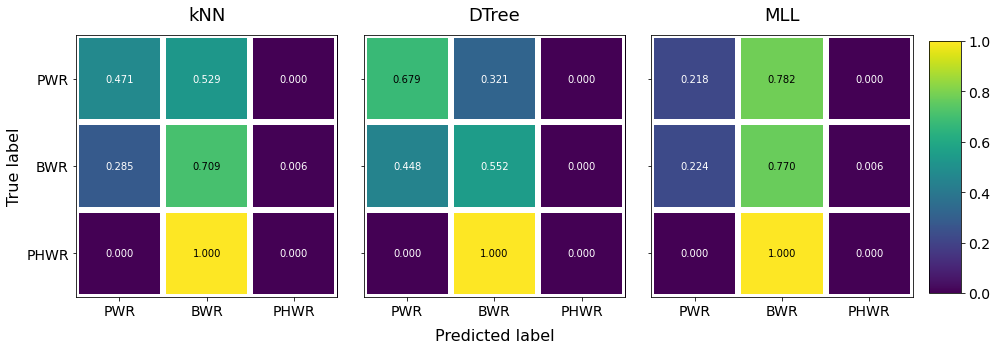
\includegraphics[width=\textwidth]{./chapters/exp1/confusion_matrix_sfco_impnull.png}
    \caption{Confusion matrices for mean-imputed null values.}
    \label{fig:cmimp}
  \end{subfigure}
  \vskip\baselineskip
  \begin{subfigure}[b]{\textwidth}
    \centering
    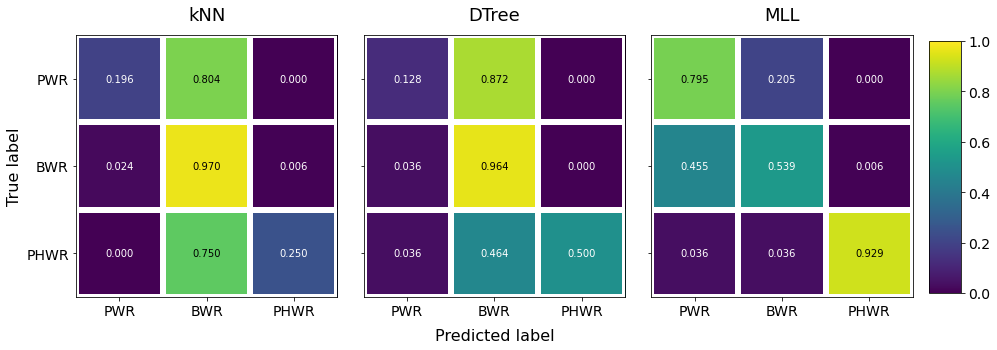
\includegraphics[width=\textwidth]{./chapters/exp1/confusion_matrix_sfco_0null.png}
    \caption{Confusion matrices for zero-replaced null values.}
    \label{fig:cm0}
  \end{subfigure}
  \caption{Confusion matrices of reactor type prediction for each algorithm 
           using two missing entry techniques: imputation with mean values 
           and replacement with zero.}
  \label{fig:cm}
\end{figure}

The expected results that \gls{MLL} will perform better with the zero-nulls test set also holds true fo

\begin{figure}[!ht]
  \centering
  \begin{subfigure}[b]{0.49\textwidth}
    \centering
    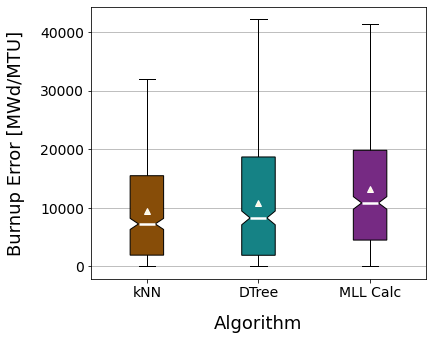
\includegraphics[width=\textwidth]{./chapters/exp1/sfcompo_boxplots_impnull_burn.png}
    \caption{imputed nulls.}
    \label{fig:burnimp}
  \end{subfigure}
  \hfill
  \begin{subfigure}[b]{0.49\textwidth}
    \centering
    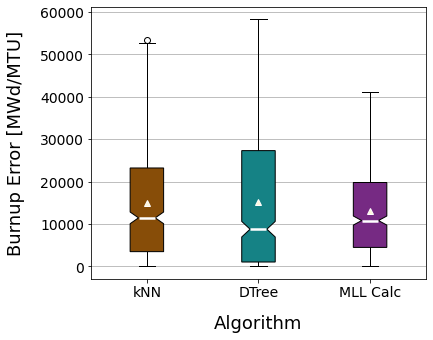
\includegraphics[width=\textwidth]{./chapters/exp1/sfcompo_boxplots_0null_burn.png}
    \caption{0 nulls.}
    \label{fig:burn0}
  \end{subfigure}
  \caption{sfcompo burnup boxplots.}
  \label{fig:sfcoburn}
\end{figure}

\begin{table}[!ht]
  \centering
  %\begin{tabular}{@{}lllllll@{}}
  \begin{tabular}{@{}m{1.5in}llllll@{}}
    \toprule
                     & \multicolumn{3}{m{2in}}{Mean Errors [GWd/MTU]} & \multicolumn{3}{c}{Median Errors [GWd/MTU]} \\ \toprule
    Null Handling    & kNN           & DTree         & MLL           & kNN            & DTree          & MLL    \\ \midrule
    Imputed Nulls    & 9.43          & 10.89         & 13.17         & 7.26           & 8.28           & 10.84  \\
    Zero-value Nulls & 14.88         & 15.18         & 3.53          & 11.47          & 8.79           & 1.70   \\ \bottomrule
  \end{tabular}
  \caption{sfcompo burnup errors.}
  \label{tbl:sfcoburn}
\end{table}

\begin{figure}[!ht]
  \centering
  \begin{subfigure}[b]{0.49\textwidth}
    \centering
    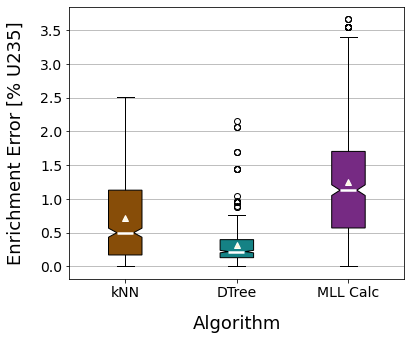
\includegraphics[width=\textwidth]{./chapters/exp1/sfcompo_boxplots_impnull_enri.png}
    \caption{imputed nulls.}
    \label{fig:enriimp}
  \end{subfigure}
  \hfill
  \begin{subfigure}[b]{0.49\textwidth}
    \centering
    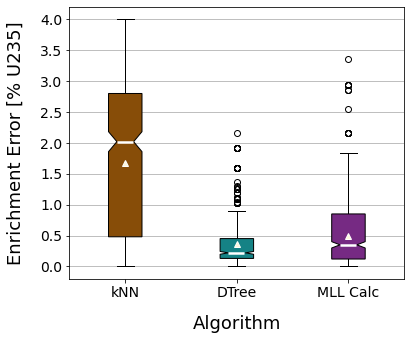
\includegraphics[width=\textwidth]{./chapters/exp1/sfcompo_boxplots_0null_enri.png}
    \caption{0 nulls.}
    \label{fig:enri0}
  \end{subfigure}
  \caption{sfcompo enrichment boxplots.}
  \label{fig:sfcoenri}
\end{figure}

\begin{table}[!ht]
  \centering
  \begin{tabular}{@{}m{1.5in}llllll@{}}
    \toprule
                     & \multicolumn{3}{m{2in}}{Mean Errors [\% U235]} & \multicolumn{3}{l}{Median Errors [\% U235]} \\ \toprule
    Null Handling    & kNN           & DTree          & MLL          & kNN            & DTree          & MLL    \\ \midrule
    Imputed Nulls    & 0.72          & 0.31           & 1.25         & 0.50           & 0.22           & 1.13   \\
    Zero-value Nulls & 1.67          & 0.36           & 0.49         & 2.02           & 0.22           & 0.35   \\ \bottomrule
  \end{tabular}
  \caption{sfcompo enrichment errors.}
  \label{tbl:sfcoenri}
\end{table}

